\documentclass[a4paper, twoside, 12pt]{article}
\usepackage[utf8]{inputenc}
\usepackage[english,french]{babel}
\usepackage[a4paper]{geometry}
\usepackage{csvsimple}
\usepackage{parskip}
\usepackage{tabulary}
\usepackage{float}
\usepackage{amssymb}
\usepackage{amsmath}
\usepackage{enumitem}
\usepackage{graphicx}
\usepackage{caption}
\usepackage{subfigure}
\usepackage{wrapfig}
\usepackage{listings}
\usepackage{stmaryrd}
\usepackage{setspace}
\usepackage{hyperref}
\usepackage{booktabs}
\usepackage{environ}
\usepackage{titlesec}
\usepackage{placeins}

\geometry{hscale=0.80,vscale=0.85,centering}

%%% Espace titres %%%

\titlespacing*{\section}{0pt}{5.5ex plus 1ex minus .2ex}{4.3ex plus .2ex}
\titlespacing*{\subsection}{0pt}{5.5ex plus 1ex minus .2ex}{4.3ex plus .2ex}
\titlespacing*{\subsubsection}{0pt}{5.5ex plus 1ex minus .2ex}{4.3ex plus .2ex}

%%% Biblio %%%

\AtBeginDocument{\setlength\bibitemsep{0.5\baselineskip}}

\usepackage[
    backend=biber,        % compilateur par défaut pour biblatex
%sorting=nyt,          % trier par nom, année, titre
    style=authoryear,
%bibstyle=alphabetic,  % style de bibliographie alphabétique
]{biblatex}
\addbibresource{bibliographie.bib}

%%% Minted + options %%%
\usepackage{minted}
\usepackage[x11names,dvipsnames,table]{xcolor}
\usepackage{colortbl}
\usepackage{mdframed}
\definecolor{bgLightGray}{RGB}{240,240,240}
\definecolor{lightgray}{gray}{.95}
\renewcommand{\theFancyVerbLine}{\normalfont {\footnotesize {\arabic{FancyVerbLine}}}}
\let\oldPYGdefault\PYGdefault
\def\PYGdefault#1#2{\hbox{\oldPYGdefault{#1}{#2}}\allowbreak{}}
\surroundwithmdframed[topline = false, leftline = true, rightline = false, bottomline = false,backgroundcolor=bgLightGray,linewidth=0.5pt]{minted}

\newcommand{\inputmintedcustom}[1]{\begingroup \catcode`_=12 \texttt{#1} \begin{mdframed}[topline = false, leftline = true, rightline = false, bottomline = false,backgroundcolor=bgLightGray,linewidth=0.5pt]
                                                                             \inputminted[linenos=true, tabsize=4, fontsize=\small, xleftmargin=0pt, xrightmargin=5pt, breaklines=true, obeytabs=true, numbersep=5mm,]{python}{#1}
\end{mdframed}}

\newenvironment{mintedcustom}
{%
    \VerbatimEnvironment
    \begin{minted}[linenos=true, tabsize=4, fontsize=\small, xleftmargin=0pt, xrightmargin=5pt, breaklines=true, obeytabs=true, numbersep=5mm]{python}%
}
{%
    \end{minted}%
    }

        \RequirePackage{luacolor}
\RequirePackage{pgf}
\definecolor{bgLightGray}{RGB}{235,235,235}
\definecolor{DarkGrey}{rgb}{0.15,0.15,0.15}
\pgfkeys{
    /consoletext/.is family, /consoletext,
    caption/.estore in = \consoletextCaption,
    label/.estore in = \consoletextLabel,
}

\newenvironment{consoletext}[1][]
{	\def\tmp{#1}%
\pgfkeys{/consoletext,#1}
\setlength{\OuterFrameSep}{0pt}						% no frame around the text
\setlength{\FrameSep}{1mm}							% just a bit of colored space around the text
\colorlet{shadecolor}{DarkGrey}                % background color to display console
    \begin{shaded}\begin{raggedright}\captionsetup{type=consoleText}\small\ttfamily\color{bgLightGray}}
    {\end{raggedright}\end{shaded}\par%
%\ifx\tmp\@nnil{\relax}\else{\vspace{-0.25cm}\captionof{consoleText}{\consoletextCaption}\vspace{0.25cm}\label{\consoletextLabel}}\fi
\ifthenelse{\equal{\tmp}{}}{}{\vspace{-0.25cm}\captionof{consoleText}{\consoletextCaption}\vspace{0.25cm}\label{\consoletextLabel}}
}


%%% Font %%%
\usepackage{fontspec}
\setsansfont{IBMPlexSans}[                       % set up custom font
    Extension = .otf,
%Path = style/fonts/,
    UprightFont = *-Light,
    BoldFont = *-SemiBold,
    ItalicFont = *-LightItalic,
    BoldItalicFont = *-SemiBoldItalic
]
\renewcommand{\familydefault}{\sfdefault}

\setlength{\parskip}{0.4em}
\setlength{\parindent}{0em}
%\setenumerate{font=\bfseries}


%%% Header & Footer %%%
\usepackage{fancyhdr}

\pagestyle{fancy}

\fancyfoot{}
\fancyhf{}

\renewcommand{\sectionmark}[1]{\markboth{\MakeUppercase{\thesection.\ #1}}{}}
%\fancyhead[RE]{\includegraphics[height=2em]{images/ichikoh.png}}
\fancyhead[RO]{\nouppercase{\texttt{\rightmark}}\sectionmark}
\renewcommand{\headrulewidth}{0pt}

\fancyfoot[LE,RO]{\texttt{\thepage}}
%\fancyfoot[RE]{\texttt{Ichikoh Industries Ltd.}}
%\fancyfoot[LO]{\texttt{Python Stress Documentation v0.9 }}   


\fancypagestyle{plain}{
    \fancyhf{}
    \fancyhead{}
    \fancyfoot{}
}

%%% Remark %%%

\makeatletter
\newenvironment{beware}[1][\@nil]
{	\def\tmp{#1}%
\setlength{\OuterFrameSep}{0pt}						% no space around the text
\setlength{\FrameSep}{1mm}							% just a bit of colored space around the text
\definecolor{shadecolor}{rgb}{1.00,0.80,0.80}		% background color for remarks
    \begin{leftbar}\noindent{}%                         % test for option or not
    \ifx\tmp\@nnil{}\else{\textbf{#1 : }}\fi}           % taken from https://tex.stackexchange.com/questions/217757/special-behavior-if-optional-argument-is-not-passed
    {\end{leftbar}\par}
\makeatother

%%% Console %%%

\definecolor{fgDarkRed}{RGB}{91,27,22}          % text color in console (draft mode)
\definecolor{fgDarkerRed}{RGB}{51,8,6}          % background color in console
\definecolor{fgVeryLightRed}{RGB}{248,226,224}

\RequirePackage{pgf}
\pgfkeys{
    /consoletext/.is family, /consoletext,
    caption/.estore in = \consoletextCaption,
    label/.estore in = \consoletextLabel,
}

%%% Paragraph %%%

\newcommand{\myparagraph}[1]{\paragraph{#1}\mbox{}\\}

%%% Titre %%%
\title{Traitement du Langage Naturel et Linguistique}

\date{M2 IAAA 2021/2022}

\author{LE BELLEGO Victor, MARTZLOFF Alice, MOUSSOX Vincent}

\begin{document}
    \maketitle
%\begin{beware}[\textcolor{red}{Important Remark}]
%\end{beware}

    \section{Certaines langues sont elles plus difficiles à analyser que d’autres ?}
    L'objectif de ce projet est d'analyser et de comprendre les raisons pour lesquelles des analyseurs syntaxiques partageant la même architecture et entraînés sur la même quantité de données obtiennent des performances très différentes sur différentes langues. On peut observer ce phénomène dans la Table 2 qui présente les performances calculées à l'aide des mesures LAS (Labeled Accuracy Score) et UAS (Unlabeled Accuracy Score) obtenues par un analyseur sur 36 langues différentes.

    \begin{table}[!h]
        \centering
        %\rowcolors{2}{bgLightGray}{}
        \begin{tabular}{ccc|ccc|ccc}
            \toprule
            \textbf{lang} & \textbf{las} & \textbf{uas} & \textbf{lang} & \textbf{las} & \textbf{uas} & \textbf{lang} & \textbf{las} & \textbf{uas} \\
            \midrule
            da & 66.18 & 73.06 & zh & 46.76 & 55.60 & pl & 68.76 & 80.69 \\
            hr & 58.88 & 69.67 & lv & 51.46 & 59.32 & sv & 64.52 & 71.11 \\
            id & 69.99 & 75.63 & he & 64.82 & 70.06 & cs & 69.77 & 77.40 \\
            ar & 60.88 & 69.78 & ko & 46.06 & 55.00 & nl & 54.92 & 63.69 \\
            eu & 47.94 & 58.17 & ja & 71.54 & 82.71 & hu & 57.21 & 69.24 \\
            it & 74.82 & 81.01 & ca & 64.79 & 71.13 & bg & 68.08 & 78.14 \\
            fa & 47.70 & 56.17 & en & 66.57 & 71.22 & vi & 48.40 & 49.62 \\
            es & 66.09 & 71.01 & pt & 70.84 & 74.55 & sl & 49.46 & 61.51 \\
            ro & 57.23 & 68.61 & et & 59.04 & 73.09 & nno & 73.58 & 78.30 \\
            de & 58.12 & 64.19 & fr & 68.40 & 73.46 & nob & 66.22 & 73.93 \\
            hi & 64.03 & 72.54 & el & 69.96 & 76.58 &  &  &  \\
            \bottomrule
        \end{tabular}
        \caption{LAS/UAS calculées pour les différentes langues (sans les \textit{configurational features})}
        \label{tab:lasuas}
    \end{table}

    \FloatBarrier

    \subsection{Variables explicatives}

    Nous faisons l'hypothèse qu'il est possible de prédire les capacités d'un analyseur entraîné sur une langue à partir de variables directement observables. La pluspart sont observées sur le corpus d'apprentissage, mais nous utilisons aussi un score de complexité à partir du WALS.

        \subsubsection{Observations effectuées sur le corpus d'apprentissage}
Ces variables observables sur le corpus sont les suivantes :

    \begin{itemize}
        \item Taille du vocabulaire
        \item Longueur moyenne d'une phrase
        \item Longueur moyenne d'un mot
        \item Taux de projectivité
        \item Longueur moyenne des dépendances
        \item Nombre moyen de dépendances
        \item Longueur moyenne de la plus longue dépendance
    \end{itemize}

\myparagraph{Taux de projectivité}

    La projectivité est une proprieté de certains arbres de dépendance. Elle se traduit par le fait que lorsqu’on trace les dependances au dessus des mots de la phrase, il n’y a jamais de croisement.

    \begin{figure}[!h]
        \centering
        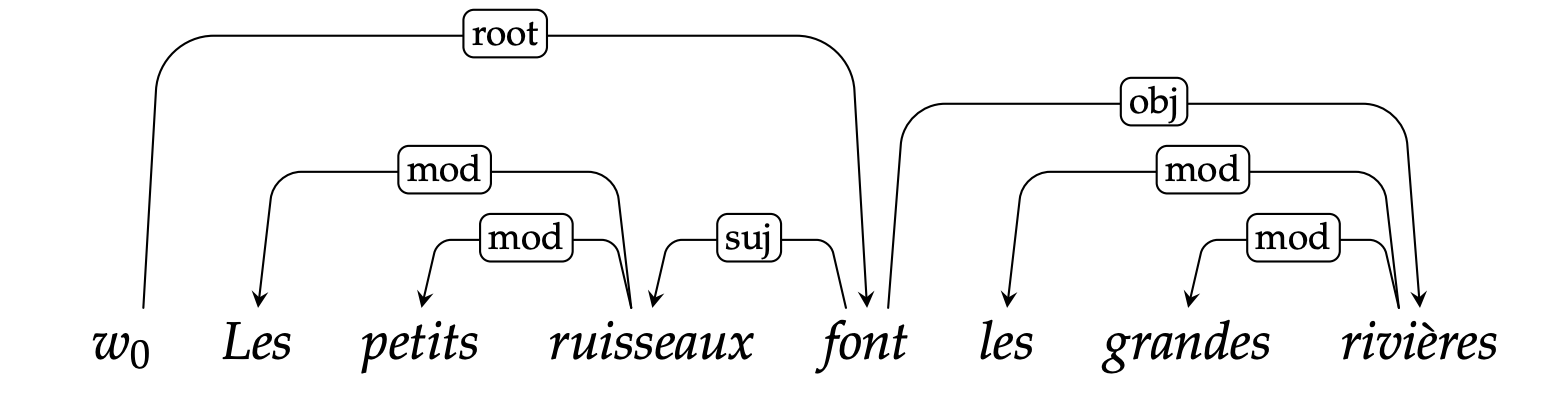
\includegraphics[width = 0.7\textwidth]{images/projectivite}
        \caption{Exemple d'une phrase française projective}
        \label{fig:projectiv}
    \end{figure}

    La grande majorité des phrases françaises sont projectives, mais il existe certains cas de non projectivité.

    \begin{figure}[!h]
        \centering
        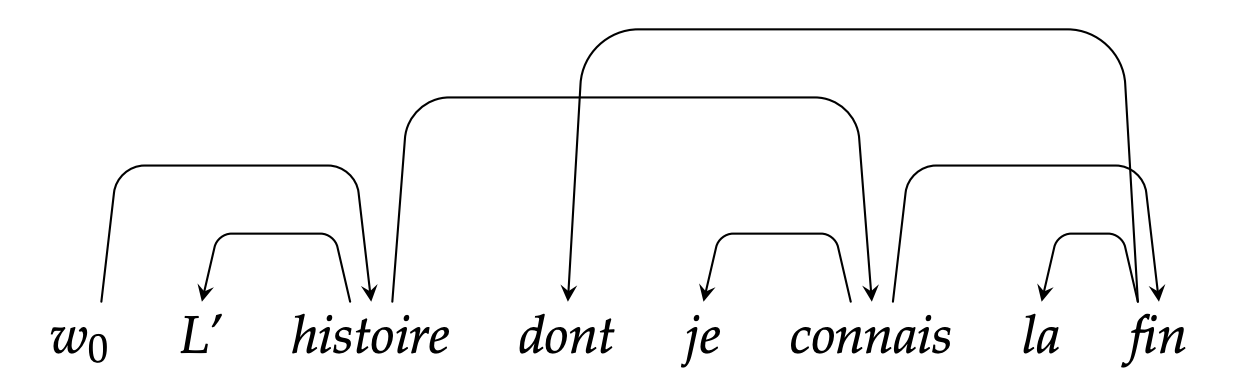
\includegraphics[width = 0.7\textwidth]{images/nonprojectivite}
        \caption{Exemple d'une phrase française non projective}
        \label{fig:nonprojectiv}
    \end{figure}

    Le degré de non projectivité varie d'une langue à l'autre. Il est elevé pour le tchèque, le néerlandais ou le turc, par exemple.

    Nous supposons que le taux de non projectivité peut expliquer les performances d'un analyseur.

    Le calcul du taux de projectivité est très simple. Il suffit de compter, pour une langue, le nombre de phrases contenues dans le fichier \texttt{lang.conllu} et le nombre de phrases contenues dans le fichier \texttt{lang\_proj.conllu} (qui ne contient que les phrases projectives) et d'en faire le quotient (voir la fonction \texttt{taux\_projectvite()} du fichier \texttt{featuresAnalyser.py} en annexe)

\myparagraph{Longueur des dépendances}

    Nous supposons que la longueur des dépendances des phrases projectives ou non projectives peut aussi expliquer les performances de l'analyseur.

Pour calculer la longueur des dépendances, nous utilions les fichiers \texttt{.mcf} et la fonction \texttt{long\_dependances()} (voir \texttt{featuresAnalyser.py} en annexe). L'agorithme opère de la manière suivante :
    \begin{enumerate}
        \item découpage des phrases grâce à l'attribut EOS (\textit{End Of Sentence})
        \item création liste de listes contenant l'attribut GOV (positions relatives des gouverneurs pour chaque mot)
        \item conversion de ces postions relatives en positions absolues grâce à la fonction \texttt{rel2abs()}
        \item création de l'arbre correspondant pour chaque liste grâce à la fonction \texttt{maketree()}
        \item calcul de la profondeur de l'arbre
    \end{enumerate} ~\par

    Nous avons extrait 3 variables explicatives pour chaque langue :
    \begin{itemize}
        \item Longueur moyenne des dépendances
        \item Nombre moyen de dépendances par phrase
        \item Longueur moyenne de la plus longue dépendance de chaque phrase
    \end{itemize}

\begin{table}[!h]
    \centering
    %\rowcolors{2}{bgLightGray}{}
    \begin{tabulary}{\textwidth}{CCCCCCCC}
        \toprule
        \textbf{lang} & \textbf{Taille du vocabulaire} & \textbf{Taille moyenne des phrases} & \textbf{Longueur moyenne des mots} & \textbf{Taux de non  projectivité} & \textbf{Nombre moyen de dépendances} & \textbf{Longueur moyenne des dépendances} & \textbf{Longueur de la plus longue dépendance} \\
        \midrule
        da & 3545 & 15.71 & 7.62 & 0.2 & 10.77 & 3.15 & 4.56 \\
        hr & 3974 & 19.2 & 7.65 & 0.08 & 13.06 & 3.64 & 5.59 \\
        id & 3580 & 18.72 & 7.4 & 0.04 & 12.64 & 3.66 & 5.59 \\
        ar & 5304 & 36.68 & 6.43 & 0.09 & 17.07 & 5.04 & 7.83 \\
        eu & 2772 & 11.39 & 7.31 & 0.34 & 7.26 & 2.76 & 4.01 \\
        it & 3354 & 20.23 & 8.06 & 0.05 & 13.34 & 3.49 & 5.11 \\
        nno & 2161 & 14.9 & 7.42 & 0.08 & 10.87 & 3.11 & 4.59 \\
        fa & 3904 & 24.02 & 5.42 & 0.07 & 14.64 & 3.78 & 6.11 \\
        es & 3424 & 25.63 & 7.58 & 0.08 & 17.69 & 3.93 & 5.94 \\
        ro & 3767 & 20.01 & 7.01 & 0.12 & 13.52 & 3.75 & 5.75 \\
        de & 4121 & 16.38 & 9.1 & 0.11 & 11.5 & 3.18 & 4.52 \\
        hi & 2453 & 19.43 & 5.33 & 0.14 & 12.14 & 3.44 & 5.0 \\
        zh & 4289 & 21.62 & 1.99 & 0.0 & 15.34 & 3.45 & 5.25 \\
        lv & 3359 & 11.68 & 7.34 & 0.08 & 8.39 & 2.98 & 4.15 \\
        he & 6050 & 29.75 & 5.16 & 0.01 & 15.49 & 3.99 & 6.18 \\
        ko & 10283 & 10.42 & 3.63 & 0.12 & 5.72 & 3.39 & 4.55 \\
        ja & 4034 & 20.18 & 2.51 & 0.0 & 14.74 & 3.54 & 5.36 \\
        ca & 2904 & 27.82 & 7.41 & 0.09 & 18.93 & 3.99 & 6.13 \\
        en & 3375 & 14.61 & 6.57 & 0.08 & 10.32 & 3.07 & 4.4 \\
        pt & 3980 & 23.93 & 7.5 & 0.13 & 15.18 & 3.75 & 5.55 \\
        et & 3683 & 8.71 & 7.31 & 0.09 & 6.55 & 2.56 & 3.4 \\
        fr & 3351 & 23.27 & 7.53 & 0.12 & 15.5 & 3.61 & 5.43 \\
        el & 2734 & 21.28 & 7.86 & 0.11 & 13.76 & 3.82 & 5.63 \\
        pl & 4762 & 8.51 & 7.79 & 0.01 & 6.09 & 2.85 & 3.9 \\
        sv & 4451 & 14.83 & 7.66 & 0.11 & 9.79 & 3.11 & 4.51 \\
        cs & 4875 & 15.52 & 7.35 & 0.13 & 10.22 & 3.45 & 5.02 \\
        nl & 3552 & 12.52 & 7.62 & 0.27 & 7.73 & 2.82 & 3.75 \\
        hu & 3677 & 19.69 & 8.05 & 0.23 & 12.5 & 3.37 & 5.1 \\
        nob & 2155 & 13.1 & 7.41 & 0.08 & 9.42 & 3.05 & 4.42 \\
        bg & 3736 & 11.68 & 7.8 & 0.03 & 8.4 & 3.19 & 4.42 \\
        vi & 1798 & 12.36 & 3.42 & 0.02 & 8.81 & 3.1 & 4.68 \\
        sl & 4219 & 13.38 & 7.3 & 0.14 & 9.34 & 2.97 & 4.2 \\
        \midrule
        moy & 3863 & 18.04 & 6.73 & 0.10 & 11.77 & 3.41 & 5.02 \\
        \bottomrule
    \end{tabulary}
    \caption{Synthèse des variables explicatives pour les corpus \textit{train} pour chaque langue}
    \label{tab:varexp}
\end{table}

    \FloatBarrier

    \subsubsection{Complexité selon M. Parkvall}

    Dans son papier \textit{The simplicity of creoles in a cross-linguistic perspective} (\cite{parkvall}) sorti en 2008, Mikael Parkvall s’intéresse à quantifier la complexité des langues. Il part du postulat qu’une expression est d’autant plus complexe qu’elle implique de règles, c’est-à-dire qu’elle requiert une longue description. Ainsi, l'hypothèse de base de l’auteur est la suivante : une langue complexe est une langue avec des constructions plus complexes. Il explore un aspect de complexité structurelle.

    Prenons par exemple la voix passive. Lorsqu’elle existe dans une langue, il faut pouvoir définir comment passer de la voie active à la voix passive, ce qui exige une explication de règle supplémentaire. Une langue qui possède une voix passive est donc, en ce qui concerne cette construction spécifique, plus complexe qu’une autre n’en possédant pas. Si on énumère donc un grand nombre de \og constructions complexes \fg{}, la langue la plus complexe sera celle qui en compte le plus grand nombre.

    Pour extraire les \og constructions complexes \fg{} qu’on peut trouver dans une langue, Parkvall utilise le set de données \textit{World Atlas of Linguistic Structures} (WALS) publié en 2005 par Haspelmath et al. Il choisit 155 langues parmi plus de 2 500, et 47 caractéristiques parmi plus de 140.

    \myparagraph{Choix des caractéristiques}

    Parkvall exclut des caractéristiques selon un raisonnement défendu dans son papier et qui s’efforce de mettre la majorité des linguistes d’accord sur le fait qu’une caractéristique apporte ou non de la complexité. Il retient les caractéristiques suivantes : \par

    \begin{table}[!h]
        \centering
        \rowcolors{2}{bgLightGray}{}
        \begin{tabulary}{\textwidth}{LLL}
            \toprule
            \multicolumn{3}{c}{\textbf{Caractéristiques du WALS}} \\
            \midrule
            Size of consonant inventories & Distance contrast in demonstratives & Morphological imperative \\
            Size of vowel quality inventories & Gender in pronouns & Morphological optative \\
            Phonemic vowel nasalization & Politeness in pronouns & Grammaticalized evidentiality distinctions \\
            Complexity of syllable structure & Person marking on adpositions & Both indirect and direct evidentials \\
            Tone & Comitative ≠ instrumental & Non-neutral marking of full NPs \\
            Overt marking of direct object & Ordinals exist as a separate class beyond ‘first’ & Non-neutral marking of pronouns \\
            Double marking of direct object & Suppletive ordinals beyond ‘first’ & Subject marking as both free word and agreement \\
            Possession by double marking & Obligatory numeral classifiers & Passive \\
            Overt possession marking & Possessive classification & Antipassive \\
            Reduplication & Conjunction ‘and’ ≠ adposition ‘with’ & Applicative \\
            Gender & Difference between nominal and verbal conjunction & Obligatorily double negation \\
            Number of genders & Grammaticalized perfective/imperfective & Asymetric negation \\
            Non-semantic gender assignment & Grammaticalized past/non-past & Equative copula ≠ Locative copula \\
            Grammaticalized nominal plural & Remoteness distinctions of past & Obligatorily overt equative copula \\
            Definite articles Indefinite articles & Morphological future &  \\
            Inclusivity (in either pronouns or verb morphology) & Grammaticalized perfect &  \\
            \bottomrule
        \end{tabulary}
        \caption{Liste des caractéristiques extraite directement du WALS}
        \label{tab:0}
    \end{table}

    \FloatBarrier

    Il ajoute à ces caractéristiques, d’autres données \og résiduelles \fg{} d’auteurs contributeurs au WALS. Ce sont les suivantes : \par

    \begin{table}[!h]
        \centering
        \rowcolors{3}{bgLightGray}{}
        \begin{tabulary}{\textwidth}{LLL}
            \toprule
            \multicolumn{3}{c}{\textbf{Caractéristiques d'auteurs du WALS}} \\
            \midrule
            Demonstratives marked for number & Demonstratives marked for gender & Demonstratives marked for case \\
            Total amount of verbal suppletion & Alienability distinctions &  \\
            \bottomrule
        \end{tabulary}
        \caption{Liste de caractéristiques proposées par les auteurs du WALS}
        \label{tab:1}
    \end{table}

    \FloatBarrier

    Enfin, il s'intéresse aussi à une donnée de Harley and Ritter (2002) à laquelle il a eu accès : \par

    \begin{table}[!h]
        \centering
        \begin{tabulary}{\textwidth}{LLL}
            \toprule
            \multicolumn{3}{c}{\textbf{Caractéristique de Harley et Ritter}} \\
            \midrule
            \color{white} Total amount of verbal suppletion & Number of pronominal numbers & \color{white} Total amount of verbal suppletion \\
            %\multicolumn{3}{c}{Number of pronominal numbers} \\
            \bottomrule
        \end{tabulary}
        \caption{Une caractéristique accessible, inspirée de Harley et al. (2002)}
        \label{tab:2}
    \end{table}

    \FloatBarrier

    Les valeurs de ces caractéristiques ont toutes été traduite par l’auteur comme des valeurs comprises entre 0 et 1 :
    \begin{itemize}
        \item \og Oui \fg{} ou \og non \fg{} deviennent 0 ou 1 avec parfois l'introduction de valeurs intermédiaire 0,5;
        \item Des valeurs d'intensité comprises entre 1 et 4 sont compréssées en : 0 - 0,25 - 0,5 - 0,75 et 1;
        \item Des valeurs catégoriques comme la classification en  \og simple \fg{}, \og modérément complexe \fg{} et \og complexe \fg{} sont traduites en 0 , 0,5 et 1.
    \end{itemize}

    \myparagraph{Choix des langues}

    L’auteur s’attèle à choisir des langues dont les annotations sont le moins lacunaires possible pour les caractéristiques décrites ci-dessus. Pour une langue i donnée :
    \begin{equation}
        \text { Score }_{i}=\frac{\sum_{k=1}^{L} \text { contribution }_{k}}{L}
    \end{equation}
    où k représente une caractéristique. Chaque langue comptant un nombre différent L de caractéristiques (parmi celles choisies par l'auteur) effectivement annontées pour cette langue. \par
    N.B.: en effet, de même que pour les caractéristiques que nous extrayons directement de nos données, Parkvall note que le set de données WALS n’est pas identiquement distribué : les langues ne sont pas identiquement annotées pour les caractéristiques proposées…

    \subsection{Cohérence des annotations}

    Dans leur article \textit{Divergences entre annotations dans le projet Universal Dependencies (\cite{nivre}) et leur impact sur l’évaluation de l’étiquetage morpho-syntaxique} (\cite{wisniewski}), Guillaume Wisniewski et François Yvon montrent que la dégradation des performances observée lors de l’application d’un analyseur morpho-syntaxique à des données hors domaine comme ici, d'une langue à l'autre, résulte d’incohérences entre les annotations des ensembles de test et d’apprentissage. Ils montrent qu'appliquer le principe de variation des annotations de Dickinson \& Meurers (\cite{meueres}) permet d'identifier les erreurs d’annotation et donc les incohérences et évaluer leur impact. Nous souhaitions nous inspirer de ces méthodes mais n'avons pu en raison notamment du temps qui nous manque proposer une telle amélioration\ldots


    \subsection{Mise en oeuvre}

    Nous réalisons une régression multiple à l'aide du modèle \texttt{LinearRegression} de \texttt{scikit-learn} pour prédire LAS après \textbf{normalisation} des variables explicatives.

    Il est d'abord intéressant de regarder les potentielles corrélations entre nos variables explicatives.

    \begin{figure}[!h]
        \centering
        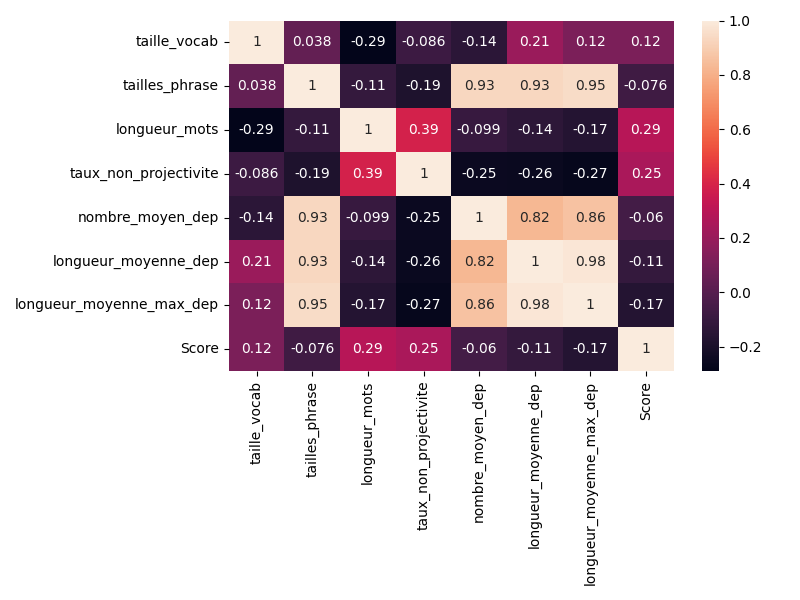
\includegraphics[width = 0.9\textwidth]{images/heatmap}
        \caption{Corrélations entre les variables explicatives}
        \label{fig:heatmap}
    \end{figure}

    \FloatBarrier

    On remarque, en toute logique, que la taille des phrases est corélée au nombre et à la taille des dépendances. On constate aussi que la longueur moyenne des dépendances est corrélée au nombre moyen des dépendances : plus il y a de dépendances, plus elles sont longues.

Nos variables normalisées sont notées comme suit :
    \begin{itemize}
        \item $x_1$ : Taille du vocabulaire
        \item $x_2$ : Longueur moyenne d'une phrase
        \item $x_3$ : Longueur moyenne d'un mot
        \item $x_4$ : Taux de projectivité
        \item $x_5$ : Longueur moyenne des dépendances
        \item $x_6$ : Nombre moyen de dépendances
        \item $x_7$ : Longueur moyenne de la plus longue dépendance
        \item $x_8$ : Score de M. Parkvall (WALS)
    \end{itemize} ~ \par

    Les LAS sont notés $y$. On souhaite estimer les $y$ tels que :
    \begin{equation*}
        \exists \left[\alpha_1,\ldots,\alpha_8,\beta\right] \in \mathbb{R},\forall i \quad y_i = \beta + \sum_{j=1}^{8} \alpha_j \cdot x_{i,j}
        \end{equation*}

    On utilise l'estimateur des moindres carrés :

    \begin{equation*}
(\hat{\alpha}, \hat{\beta})=\arg \min _{\alpha, \beta} \sum_{i=1}^{n}\left(y_{i}-\left(\alpha x_{i}+\beta\right)\right)^{2}
\end{equation*}

On obtient les résultats suivants : \par

$\beta = 61.66 $, $\alpha_1 = -2.32$, $\alpha_2 = -0.75$, $\alpha_3 = 3.63$, $\alpha_4 = -3.56$, $\alpha_5 = 3.76$, $\alpha_6 = 17,40$, $\alpha_7 = -18.33$, $\alpha_8 = 0.02$

avec $R^{2} = 0.476$, qui est moyen. L'erreur RMS s'élève à $6.198$.

    Du fait de la normalisation des variables d'entrée, il est directement possible de déduire l'impact de chaque variable. On remarque que le score de M. Parkvall (WALS) a un impact quasi nul sur la régression. En revanche, la longueur moyenne des dépendance et la longueur moyenne de la plus longue dépendance ont une importance majeur, bien qu'opposé.

    \subsection{Conclusion}

    \subsubsection{Est-il possible de connaître a priori les performances de l’analyseur en fonction de certaines caractéristiques de la langue ?}

    Bien que les résultats obtenus ne soient pas à la hauteur des espérance, il semblerait certaines caractéristiques de la langue permettent de connaître a priori les performances de l’analyseur.

    Notre étude porte sur un \textbf{corpus de faible taille qui comporte, par essence, de nombreux biais} ; il est donc difficile de généraliser. Une étude avec des corpus de plus grande taille serait nécessaire pour affiner la régression et ainsi conclure de manière plus certaine.

    \subsubsection{Est-il possible d’utiliser les conclusions de l’étude statistique pour améliorer les performances de l’analyseur ?}

    Il est a priori possible d'utiliser l'étude statistique pour améliorer les performances de l’analyseur. En effet, connaissant les caractéristiques de la langues, on peut choisir un analyseur moins sensible à la non projectivité ou aux longues dépendances, mais plus couteux seulement pour les langues qui le requierent. Les langues projectives (comme le japonais) peuvent être traités avec des analyseurs plus simples et moins coûteux.

    Ainsi, l'étude statistique permet d'améliorer les performances de l’analyseur en orientant l'investissement en ressources pour les langues les plus \og complexes \fg{}

    \printbibliography

    \clearpage

    \appendix
    \section*{Annexes}
    \inputmintedcustom{../resultsTable.py}
    \inputmintedcustom{../featuresAnalyser.py}
    \inputmintedcustom{../RegressionMultiple.py}

\end{document}